\subsection{MATLAB \& Paparazzi Simulation}
Another way to carry out a simulation is to use MATLAB for the simulation of the vision algorithm (see Figure \ref{matlab}), and Paparazzi NPS simulator for the simulation of the flight plan (see Figure \ref{paparazzi_sim}). From the MATLAB simulation results, the appropriate color and width-thresholds for the initial practical trial can be derived. Note that these thresholds can only serve as the initial values because in the end they have to be fine-tuned through real-life tests. As for the flight plan, the Paparazzi NPS simulator can be used to verify the practicability and performance of the proposed flight plan. Although this simulator can yield realistic results, it has a drawback that the simulation cannot incorporate the vision algorithm. Thus, a "fake vision result" is supplied by an NPS file which we designed as a random number generator; it gives 0, 1, and -1 as output where 0 means 'no obstacle detected', 1 means 'obstacle on the left', and -1 means 'obstacle on the right'. The frequency of the occasions when it gives 1 or -1 is adjusted in this NPS file, so that by increasing this frequency, the simulation represents the situation where there are many obstacles present.
\begin{figure}[h]
	\centering
	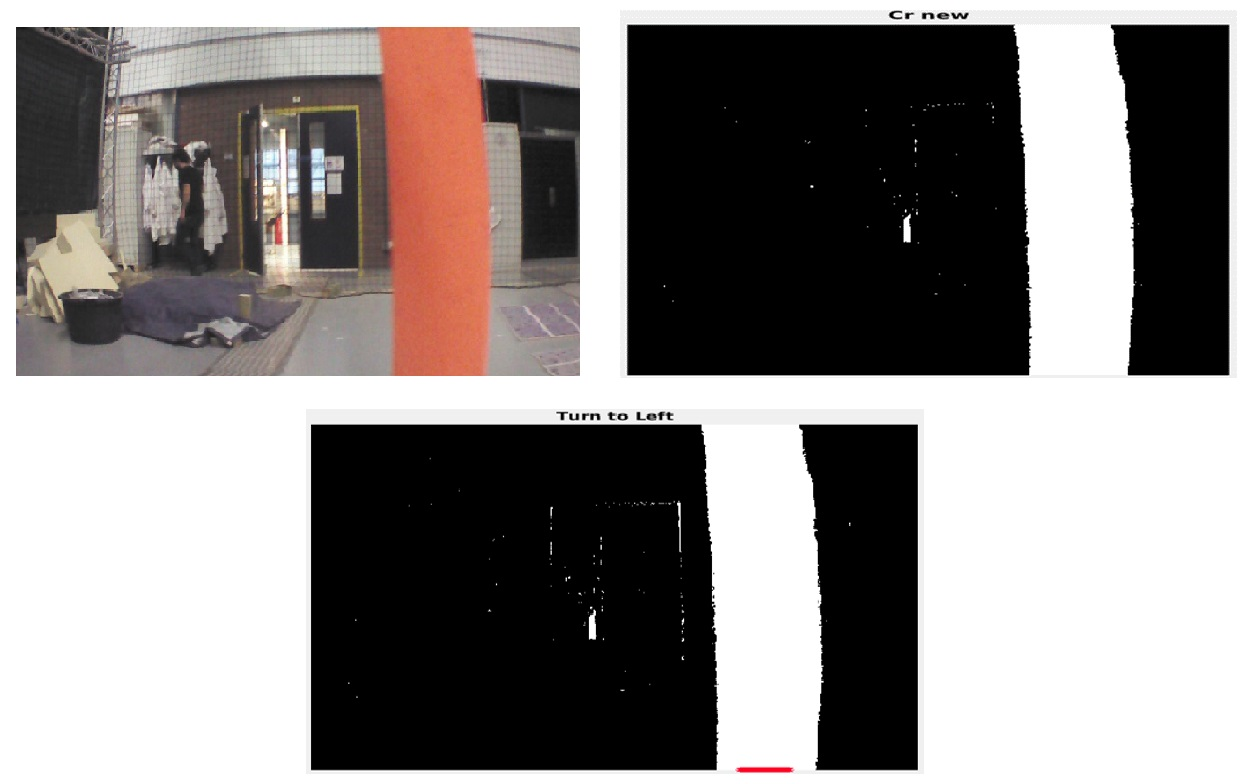
\includegraphics[width = 0.5\textwidth]{Figures/matlab.jpg}
	\caption{MATLAB simulation of vision algorithm using an image from the AR.Drone 2.0. Top left: original image captured. Top right: binary map computed using a threshold in Cr channel. Bottom: Detection of the orange pole. The red marks on the bottommost row indicate the location of the orange pole nearby.}
	\label{matlab}
\end{figure}
\begin{figure}[h]
	\centering
	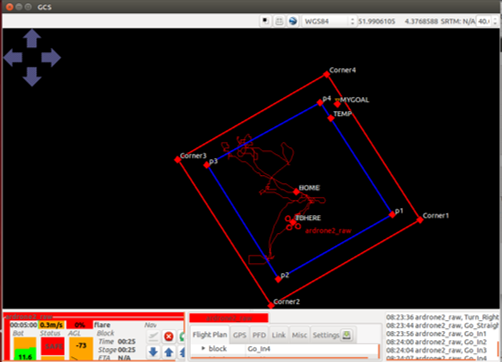
\includegraphics[width = 0.5\textwidth]{Figures/paparazzi_sim.png}
	\caption{Paparazzi simulation of the flight plan. The blue lines indicate the boundaries of the flight area.}
	\label{paparazzi_sim}
\end{figure}